%Introduction

\chapter{Introduction}
\label{sec:introduction}

%\chapter{Nucleation}
%\label{sec:nucleation}
%
\section{Nanotechnology}
\label{sec:nanotechnology}

Not many scientists can claim to have envisioned an entirely new field of
physics, but it is not an overstatement to say that the field of
\emph{nanotechnology} was developed in large parts due to one of the most
brilliant physicists of the 20th century, Richard Feynman. In his talk ``There's
Plenty of Room at the Bottom---An invitation to enter a new field of
physics''\autocite{Feynman_TherePlentyRoom_1960} he challenges scientists to
construct devices and compounds that only consist of a few tens or hundreds of
atoms. Such objects usually turn out to be a few nanometres ($10^{-9}$~m) in
diameter, giving rise to the field's name. It is astounding to read through the
transcript of Feynman's talk from today's perspective, as it is filled with
ideas that are very much a reality now. For example, he devises the
miniaturisation of the computer and even mentions the concept of a facial
recognition system. One of the reasons Feynman gives for the usefulness of this
field is cost effectiveness. Scaling everything down in size decreases the
amount of materials needed drastically. As a side effect one ends up with much
smaller and potentially more powerful devices.

Feynman noted that in order to effectively use nano-scale devices one needs to
be able to investigate these small structures down to the atomic level,
something that was not possible with the electron microscopy methods available
at the time. This became a practical reality with the invention of the \ac{STM}
in 1981,\autocite{Binnig_ScanningTunnelingMicroscopy_1986} which secured its
inventors the Nobel prize in 1986. Figure~\ref{fig:STM} shows an image produced
with such a microscope.
%
\begin{figure}[htb]
    \centering
    \subfloat[\label{fig:STM}]{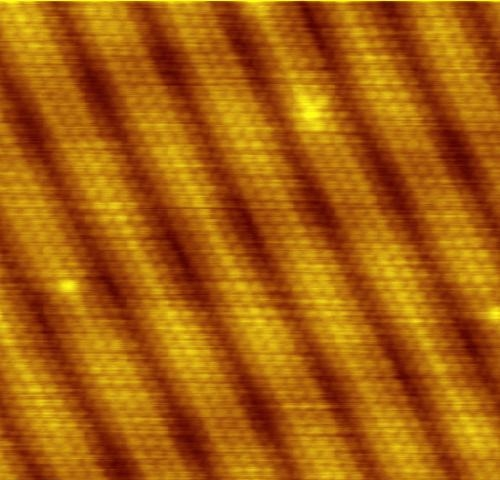
\includegraphics[width=0.35\textwidth]{other-pics/Atomic_resolution_Au100.png}}\hspace{0.05\textwidth}
    \subfloat[\label{fig:IBM}]{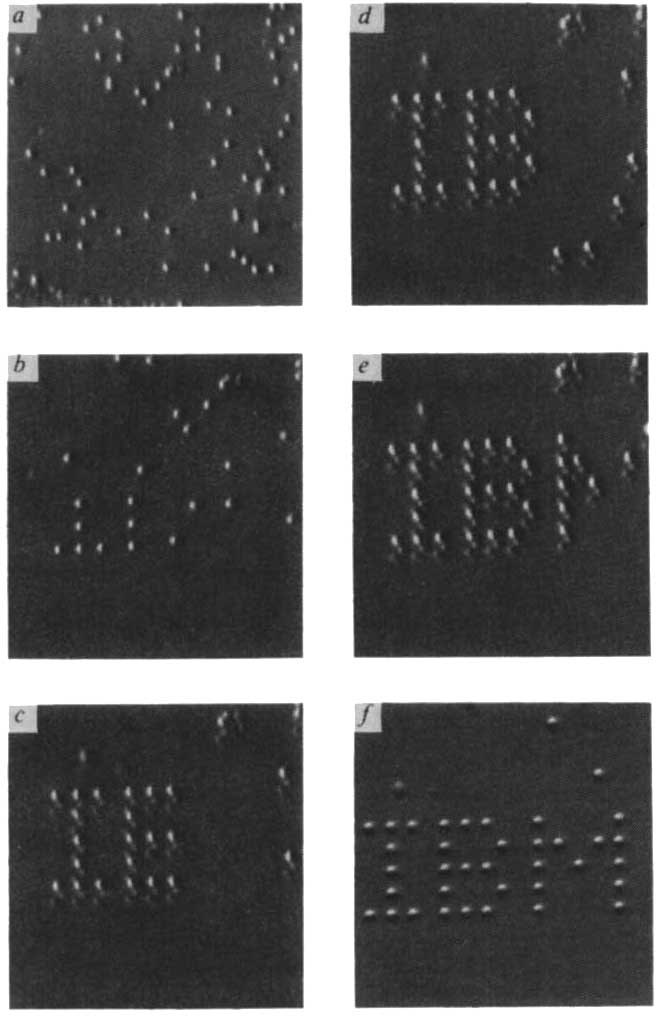
\includegraphics[width=0.35\textwidth]{other-pics/ibm.png}}
    \caption{\protect\subref{fig:STM} \acs{STM} image of a clean gold (100) surface showing atomic resolution. The ridges are a result of surface reconstructions. The image is part of the public domain. \protect\subref{fig:IBM} \acs{STM} image of Xenon atoms arranged on a nickel (110) surface in a pattern resembling the IBM logo. Reprinted by permission from Springer Nature Customer Service Centre GmbH: Springer Nature, \citetitle{Eigler_Positioningsingleatoms_1990a}\autocite{Eigler_Positioningsingleatoms_1990a}, \textcopyright 1990.}
    \label{fig:STMexamples}
\end{figure}
%
One problem with \ac{STM} imaging is that it only works on conductive surfaces.
However, this was resolved with the introduction of the \ac{AFM}, which does not
rely on a tunnelling current to produce atomic
resolution.\autocite{Binnig_AtomicForceMicroscope_1986} The technology was
perfected to such a degree that it became possible to move individual atoms and
arrange them in almost any pattern imaginable
(figure~\ref{fig:IBM}).\autocite{Eigler_Positioningsingleatoms_1990a}

In the last part of his talk, Feynman speaks about how ``atoms on a small scale
behave like nothing on a large scale, for they satisfy the laws of quantum
mechanics''. This property has found application in so-called nano-particles,
which refers to molecules or chemical compounds in general with the size of a
few nanometres. Belonging to this group are for example the
\emph{Buckminsterfullerenes} (or short fullerenes) discovered by
Kroto\autocite{Kroto_C60Buckminsterfullerene_1985} or carbon
nano-tubes\autocite{Iijima_Helicalmicrotubulesgraphitic_1991}, and their
discovery helped fuelling the push for nanotechnology even further. It was
however not until the beginning of the 21st century, that nanotechnology gained
traction by securing public funding, e.g. from the National Nanotechnology
Initiative, a U.S. American federal government program. This increase in
research funding gave rise to lots of interesting scientific projects like the
``Nanocar''\autocite{Kudernac_Electricallydrivendirectional_2011} or Graphene
transistors.\autocite{Wu_Highfrequencyscaledgraphene_2011} Today, the technology
is present in many consumer products with over 800 goods reported to contain
nanotechnology.\autocite{Vance_Nanotechnologyrealworld_2015}

\section{Cluster Science}
\label{sec:ClusterScience}

A term that is often used for chemical compounds used in nanotechnology is
\emph{cluster}, but the definition of this term is still debated. Originally, it
was proposed as ``an appropriate one [term] for a finite group of metal atoms
which are held together mainly, or at least to a significant extent, by bonds
directly between the metal atoms, even though some non-metal atoms may also be
intimately associated with the
cluster''.\autocite{Cotton_MetalAtomClusters_1964} However, this definition
limits itself only to the fraction of metal atoms in the periodic table and the
term is not necessarily used in this form today. The most accurate definition of
a cluster is perhaps given through size, as almost any chemical compound with a
finite number of atoms of $2$--$10^n$ ($n\lessapprox 7$) atoms is referred to as
a
cluster.\autocite{Johnston_Atomicmolecularclusters_2002,Wales_Energylandscapes_2003}
Therefore, clusters are structures, that are of intermediate size, bridging the
gap between small molecules and bulk solids,\footnote{It should be noted that
very large organic compounds like peptides are usually not considered clusters,
and are exempt from this definition.} and they appear naturally when discussing
nucleation phenomena and nano-particles. 

Clusters can be divided into several groups that are characterised by the type
of atoms comprising the cluster and therefore its electronic bonding situation.
For example, molecular clusters, which, due to their closed electronic shells,
mainly interact inter-molecularly via weak van-der-Waals forces. However, the
intra-molecular interactions are usually of covalent nature. Such clusters are
found for simple molecules, such as water,\autocite{Liu_WaterClusters_1996}
ammonia\autocite{Beu_Structureammoniaclusters_2001} or carbon
dioxide.\autocite{Takeuchi_GeometryOptimizationCarbon_2008} Moreover,
semi-conductor clusters are bound much more strongly by covalent interactions.
Their name stems from the type of atoms that make up the cluster as they are
semi-conductors in the solid state. Most famously, this group includes the
already mentioned carbon
fullerenes\autocite{Kroto_C60Buckminsterfullerene_1985}, but also other
semi-conductors like silicon\autocite{Zhu_Structuresstabilitiessmall_2003a} and
germanium.\autocite{Pacchioni_Silicongermaniumclusters_1986} If a cluster is not
monoatomic and the difference in the electronegativity of the atoms is large
enough the covalent bonding situation can change to ionic.

\begin{figure}[htb]
    \centering
    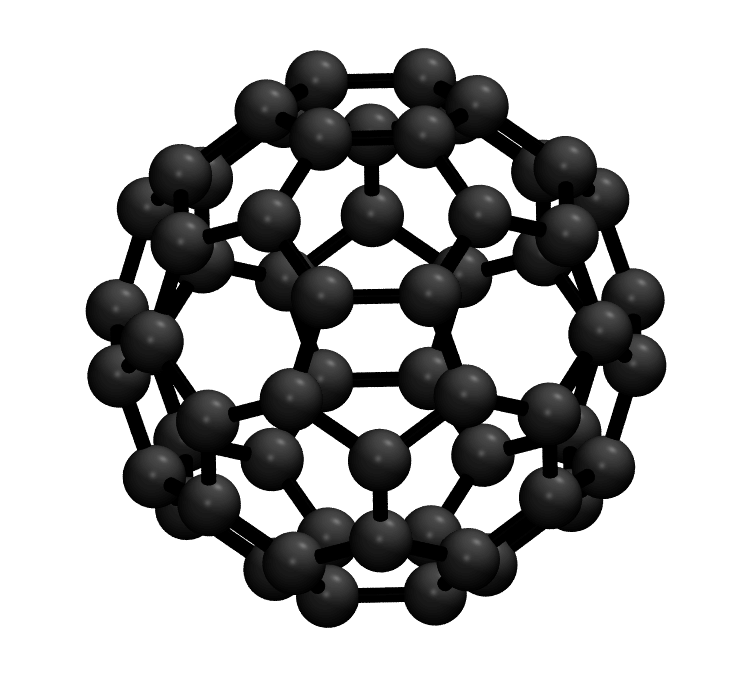
\includegraphics[width=.5\textwidth]{golddual/C60Ih.png}
    \caption{Buckminsterfullerene \ce{C60}.}
    \label{fig:C60example}
\end{figure}

For this thesis, two other types of clusters are more relevant, monoatomic metal
and rare gas clusters. The bonding situation in metal clusters is particularly
interesting, because of the high degree of delocalisation and non-directional
bonding. To describe this situation, several bonding models have been developed.
The most simple one is perhaps the \emph{liquid drop model} which approximates
the metal cluster as a uniform conducting sphere, i.e. it is a classical
electrostatic model. The liquid drop model does not give rise to an electronic
structure, which is resolved in the \textit{spherical jellium model}. In this
model the cluster is modelled as a uniform, positively charged sphere filled
with an electron gas, which is solved using the \textit{Schr\"odinger equation}.
This gives rise to quantised electron energy levels and therefore an electronic
shell structure. For metal clusters of not too many atoms it is also possible to
use accurate quantum chemical methods, which will be introduced in
chapter~\ref{sec:basicsofQC}.

Rare gas clusters can form at very low temperatures, when the average kinetic
energy of the rare gas atoms is smaller than the weak dispersive forces between
them. The reason they interact so weakly is because of their closed shell
electronic structures, allowing for neither covalent nor ionic bonding. As
dispersive interactions are a correlation effect of the electrons, it is
difficult to describe them accurately with quantum chemical methods. However,
the interaction can be approximated by simple models like, for example, the
London formula.
%
\begin{align}
    V_\text{disp}=-\frac{C_6}{r^6},\quad C_6=\frac{3\alpha^2I}{4\left(4\pi\varepsilon_0\right)^2}
\end{align}
%
Here, $I$ is the ionisation potential and $\alpha$ is the atomic polarisability.
In combination with a term describing the repulsive contribution to the energy,
the Lennard-Jones potential can be derived, which agrees well with structural
and energetic predictions for rare gas clusters. The Lennard-Jones potential
will be explained in more detail in chapter~\ref{sec:energylandscapes}.

\section{The Potential Energy Surface}
\label{sec:ThePotentialEnergySurface}

A question that naturally arises when studying clusters bound by a certain
potential is ``how many stable structures exist for a given number of atoms
$N$'' and related to this ``what is the most stable structure''. For this, it is
useful to investigate this problem from a mathematical point of view. If the
movement of the atomic nuclei is decoupled from the electronic movement
(Born-Oppenheimer approximation,
section~\ref{sec:bornoppenheimerapproximation}), the nuclei can be said to move
on a potential energy hypersurface. This \ac{PES} is a multi-dimensional
function of all $3N$ atomic coordinates and it maps each point of configuration
space to an energy value depending on the chosen potential. A stable structure
on this hypersurface corresponds to a local minimum, with the most stable
structure being represented by the global minimum. Thus, the question of how
many stable structures there are is equivalent to the question of how many local
minima can be supported by the multi-dimensional potential energy surface. An
example for such a hypersurface is shown in figure~\ref{fig:PES-3D}.
%
\begin{figure}[htb]
    \centering
    \subfloat[\label{fig:PES-3D}]{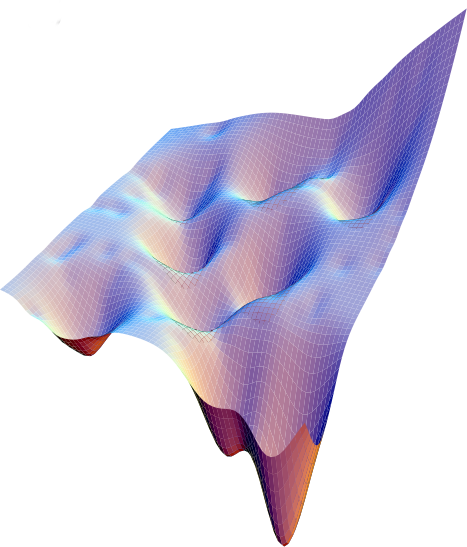
\includegraphics[width=0.375\textwidth]{other-pics/PES-3D.png}}\hspace{0.05\textwidth}
    \subfloat[\label{fig:PES-2D}]{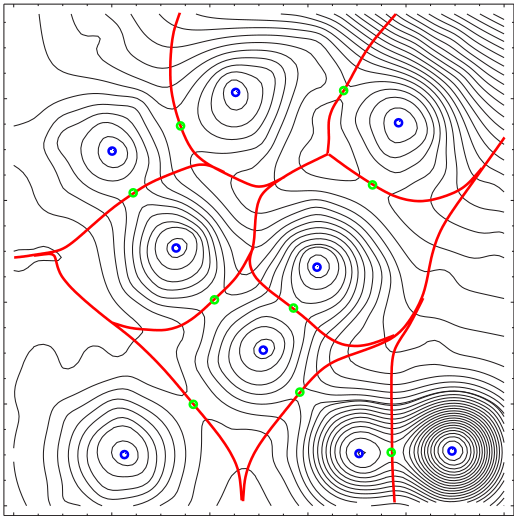
\includegraphics[width=0.375\textwidth]{other-pics/PES-2D.png}}
    \caption{\protect\subref{fig:PES-3D} Example of a two-dimensional potential energy landscape and \protect\subref{fig:PES-2D} the same hypersurface represented with contour lines. Red lines mark the boundaries of the basins of attraction around the minima (blue dots) and transition states (green dots). Reprinted figures with permission from the American Physical Society: \citetitle{Massen_Powerlawdistributionsareas_2007}\autocite{Massen_Powerlawdistributionsareas_2007}, \textcopyright 2007 by the American Physical Society.}
    \label{fig:PES}
\end{figure}
%
The distribution of the minima on the hypersurface can be investigated by
dividing the configuration space into basins of attraction as shown in
figure~\ref{fig:PES-2D}. A basin of attraction marks an area (or hyper-area for
multi-dimensional \acp{PES}) in which the enveloped minimum (blue dots) can be
reached from any point of configuration within the basin of attraction by
following a steepest-descent path. These basins of attraction therefore tile the
energy landscape, and it was found that this tiling is very similar to that of
Apollonian packings.\autocite{Massen_Powerlawdistributionsareas_2007} The
results also suggested that this is a universal feature of \acp{PES},
independent of the underlying potential. Furthermore, the area of the basins
seems to correlate with the depth of the corresponding minimum, which makes
finding the global minimum on a \ac{PES} a little bit easier as it should
correspond to the largest basin of attraction by area.

The question of stable structures can also be tackled from a different point of
view, namely that of graph theory. Under the assumption that the atoms in a
cluster are connected, the question becomes ``how many non-isomorphic connected
graphs exist for a specific number of vertices $N$''. This problem is also known
as the Graph isomorphism problem and no analytic solution is known. However, it
can be attempted to derive upper and lower bounds within which the solution must
lie. As graphs can be represented by adjacency matrices
(chapter~\ref{sec:DefinitionGraph}), the maximum number of such matrices can be
used as a loose upper bound, i.e.
$2^{N(N-1)/2}=\mathcal{O}\left(\exp{N^2}\right)$ different matrices
exist.\autocite{Arkus_Minimalenergyclusters_2009} Some observations
suggest\autocite{Tsai_Useeigenmodemethod_1993} that the growth is exponential,
to be precise asymptotically
exponential.\autocite{Stillinger_Packingstructurestransitions_1984,Stillinger_Exponentialmultiplicityinherent_1999}
\\\newline
Another interesting question with special importance for chemistry is the number
of contacts or bonds a cluster can form. This question is fundamentally linked
to the Gregory-Newton problem, which asks ``how many spheres can be arranged
around a central sphere of the same size such that they all touch the central
sphere''. As proven by
\citeauthor{Schutte_ProblemdreizehnKugeln_1952}\autocite{Schutte_ProblemdreizehnKugeln_1952}
there can be no more than 12 spheres satisfying these conditions simultaneously.

\section{Outline}
\label{sec:Outline}

I this thesis, three projects, in which clusters are investigated with both
mathematical and physical models, will be presented.

In the first project (chapter~\ref{sec:goldendualfullerenes}), a special type of
metal clusters is investigated. The gold clusters are hollow triangulations of
spheres and can therefore be created by wrapping a cut-out from a (111)
face-centred cubic sheet of gold around a sphere. Graph-theoretically, they are
related to fullerenes as they represent their geometric duals. The structures
and energies of the clusters are investigated with quantum mechanical methods
and their growth behaviour is examined. Furthermore, photoelectron spectra are
simulated and compared to previous experimental results.

The second project (chapter~\ref{sec:fromstickyhardspheretoLJtypeclusters}) is
concerned with the investigation of a relation between two interaction
potentials employed in cluster science. The first one is the \ac{SHS} potential,
which is not continuous, thus the stable clusters have to be searched by means
of graph theoretical methods through the adjacency relation. The form of this
potential represents the mathematical limit of the \ac{LJ} potential with
respect to the exponents approaching infinity. Starting from the structures from
the sticky hard sphere potential geometry optimisations are carried out with
\ac{LJ} potentials with growing exponents and investigated with respect to the
convergence of the total number of unique structures towards the \ac{SHS} limit
and their asymptotic exponential growth behaviour.

In the last project (chapter~\ref{sec:thegregorynewtonclusters}), the special
case of the Gregory-Newton clusters is revisited. First, the question is posed
if very soft (small exponents) \ac{LJ} potentials allow a 13th sphere to pack
with equal distance around a central sphere. The set of \ac{SHS} clusters is
again used as a starting point for the next part. It is searched for
Gregory-Newton type clusters, which are then analysed by graph theoretical
means. The aim was to understand if the graphs spanned by the 12 surrounding
spheres are sub-graphs of the icosahedral graph. The reason for this
investigation is linked to the fact that under the conditions of the sticky hard
sphere potential icosahedral symmetry cannot be realised. However, this is known
to be a very stable structural motif for \ac{LJ} systems. Therefore, the point
at which the symmetry of the \ac{PES} breaks and the Icosahedron is not
supported by the \ac{PES} is investigated. Finally, the set of \ac{SHS} clusters
was analysed for Gregory-Newton clusters where one sphere enters the second
coordination shell. Here, the focus was put on finding the shortest distance
this sphere can have to the central sphere.



%
%As the clusters grow in size, their properties become more and more bulk-like,
%because the electronic states are no longer quantised but quasi-continuous.
%Understanding these growth behaviours could help to unravel questions around
%crystal growth or at which size metallic conductivity can be first observed. 
%
%In this thesis, three projects related to cluster science, are investigated.
%First, the theoretical background required to carry out the calculations will be
%reviewed and a quick overview of the program package \textsc{Spheres} developed
%in this thesis will be given. The final three sections contain the results of
%the investigations. A special type of hollow gold clusters will be investigated
%in chapter~\ref{sec:goldendualfullerenes} with respect to their geometry and
%stability. These clusters show an interesting connection to the carbon
%fullerenes. Rare gas clusters are subject of
%chapters~\ref{sec:fromstickyhardspheretoLJtypeclusters} and
%\ref{sec:thegregorynewtonclusters}. The investigations in these chapters are
%focused on clusters interacting via interaction potentials that describe
%dispersive effects. The last chapter also uses graph theoretical methods to
%investigate the connectivity of the clusters with respect to the Icosahedron.
%Each project will be introduced more thoroughly in the beginning of the
%respective chapter.

